\documentclass{article}
\usepackage{datatool, xcolor, listings, graphicx}
\usepackage[utf8]{inputenc}
\usepackage{xcolor}

\DTLsetseparator{;}
\DTLloaddb{uicontrols}{data.csv}

\begin{document}
\lstset{backgroundcolor=\color{lightgray}}
%get the value of Text Column provided ID Cancel_confirmation_header
%\DTLfetch{uicontrols}{ID}{Cancel_confirmation_header}{Text}
%define a new macro to get the value of the Text Column provided the ID in the argument
\newcommand{\uicontrol}[1]{\textcolor{blue}{\textbf{\DTLfetch{uicontrols}{ID}{#1}{Text}}}}

\section*{Aborting the process}
Errors in the performance of the process can be observed early in the execution. Aborting the process early and correcting the errors in the script saves time. This task describes how to abort a running process.  
\begin{description}
	\item[Prerequisite] A running process
	\item[Prerequisite] Administrator user rights. 
\end{description}
\begin{enumerate}
	\item From the command line start the administrators console
	\begin{lstlisting}[frame=single]
C:\> acme_ad_cosole
	\end{lstlisting}
	\item Go to \uicontrol{AdminConsole_ProcessOverview} $>$ \uicontrol{AdminConsole_Running}
	\item Choose the \uicontrol{AdminConcole_AbortProcess} option
	\item In the \uicontrol{Cancel_confirmation_header} dialog, confirm with \uicontrol{Cancel_confirmation_cancel_button}\\[1ex]
	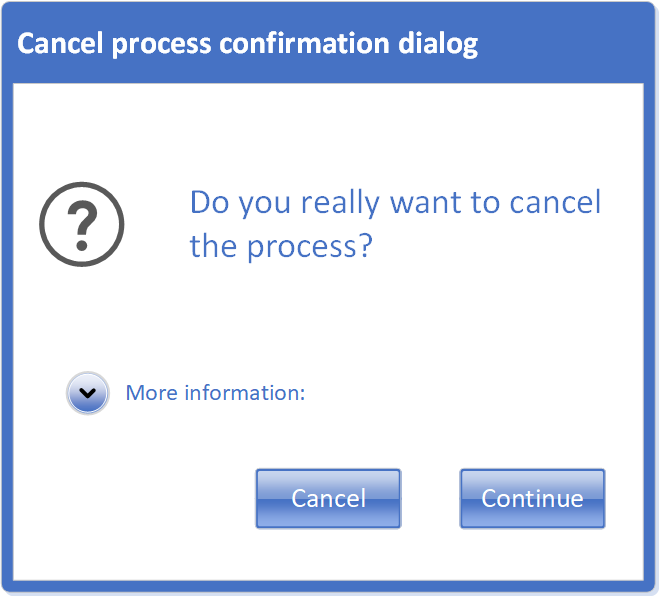
\includegraphics[width=0.5\textwidth]{cancel_process}
	\begin{itemize}
		\item The process is aborted
	\end{itemize}
\end{enumerate}
\end{document}